\documentclass{article}

\usepackage{amsmath}
\usepackage{amssymb}
\usepackage{graphicx}
\usepackage{subfigure}
\usepackage[shortlabels]{enumitem}
\usepackage{geometry}
\usepackage{float}
\usepackage{caption}
\usepackage{amsmath}
\usepackage{listings}

\geometry{left=3.5cm,right=3.5cm,top=3.0cm,bottom=3.0cm}

\begin{document}

\title{Cross-match between APOGEE and TGAS catalog based on KDTree algorithm}
\author{Shengqi Yang}
\maketitle

\begin{center}
\textbf{Abstract}\par
\end{center}
\par
\parindent=19pt
	This paper introduced a simplified KDTree model compared to Scipy KDTree. It only handles cross-match between two dimensional data sets. The first part is a brief introduction of data sets used in this work: APOGEE and TGAS catalog. The second part is an overview of KDTree algorithm applied in the program. The third part compares cross-match results given by self-defined KDTree and Scipy KDTree. The fourth part displays assessments of this simplified method and possible improvements.\par
\vspace{12pt}

\textbf{Introduction of APOGEE and TGAS catalog}\par
\vspace{12pt}
	APO Galactic Evolution Experiment (APOGEE) is a survey contains information of 155632 red giant stars in Milky Way Galaxy, including high-resolution, high signal-to-noise position, bands magnitudes and so forth. \par
	The Tycho-Gaia Astrometric Solution (TGAS) is another survey contains information about 2057050 stars in Tycho-2 catalogue, including their positions, parallaxes, proper motions and so forth.\par
	Generally speaking, these two surveys are focusing on different stars on sky. However, they do have an overlapping part. We are interested in stars of this region and want to find them out for further usage.\par
	Due to the large volume of these two data sets, it is inconvenient and unnecessary to pick matching pairs through enumeration method. Here I use KDTree and midpoint-split method to realize highly efficient cross-match.\par

\vspace{12pt}
\textbf{Overview of KDTree algorithm.}\par
\vspace{12pt}
	Cross-match is actually to pair one star in APOGEE and one star in TGAS with very similar position coordinates: RA (right ascension) and DEC (declination). The ideal is to use all the data in one catalog (say APOGEE) to build special data structure (KDTree) and use data in another catalog (TGAS) to inquiry it and find the matching point in the first catalog quickly.\par
	 To build the KDTree, firstly I define a class called node():
	 \begin{lstlisting}
class node:
    def __init__(self):
        self.l=[]
        self.r=[]
        self.split='NAN' #Record the spliting point
        self.divdim='NAN' #Record which dimension to be splited
    def set_left(self,data):
        self.l=data
    def set_right(self,data):
        self.r=data
    def set_split(self,split):
        self.split=split
    def set_divdim(self,divdim):
        self.divdim=divdim
    \end{lstlisting}\par
    Starting from the whole data set, compute the length: $max(RA)-min(RA)$ and midpoint: $\frac{max(RA)+min(RA)}{2}$ of RA. Do the same thing to DEC data. Then apply midpoint-split method to decide the hyperplane. Specifically speaking, choose the dimension of highest length to split, assign data with value less than the midpoint to left branch, others to the right branch. Record the dimension index as well as the midpoint value and repeat this branching process (through recursion) until the data volume in one branch is less than the leaf size ($leafsize=10$ in this program). Thus every data of APOGEE is in a certain leaf of a tree like data structure. The main branching process is realized through recursion and is shown below:\par
    \begin{lstlisting}
def kdtree(data):
    if data.shape<=leafsize :  
        return data
    else:
        branch=node()
        data_l=data value less than median
        data_r=data value no less than median
        branch.set_left(kdtree(data_l))
        branch.set_right(kdtree(data_r))
        return branch
    \end{lstlisting}\par
    The second step is to pour TGAS data into this tree and let the data points flow along tubes following the same rule in the first step. i.e. Say $node.split==i$ and $node.divdim==j$, if a point's A[j] is less than i, it flows into the left branch, otherwise to the right branch. Finally point A comes to a leaf which contains at most 10 data points. It is far more easier to find a neighbor in 10 data instead of 155632.\par
    Neighbor is two points with very small separation, but one have many ways to define the "distance". To stay consistent with cross-match code in astropy, here I use angular separation:
        $$\theta=\left(\dfrac{180}{\pi}\right)tan^{-1}\left(\dfrac{\sqrt{cos^2\sigma_2sin^2(\alpha_2-\alpha_1)+[cos\sigma_1sin\sigma_2-sin\sigma_1cos\sigma_2cos(\alpha_2-\alpha_1)]^2}}{sin\sigma_1sin\sigma_2+cos\sigma_1cos\sigma_2cos(\alpha_2-\alpha_1)}\right)$$\\
     $\sigma_i$ are declination of the $i^{th}$ point in radians. \\
     $\alpha_i$ is the right ascension of the $i^{th}$ point in radians. \\
     $\theta$ is the angular separation between two points in degree.\par
     If the minimum angular separation between A and all the data in the KDTree leaf is smaller than 2 arcsec, the corresponding point in APOGEE is defined as its' matching point.\par
	 
\vspace{12pt}
\textbf{Result and comparison.}\par
\vspace{12pt}
	Since constructing KDTree is time consuming, I use the samller catalog APOGEE to build KDTree and use TGAS data to inquiry it. Scipy KDTree finds 20113 pairs of matching points in APOGEE and TGAS catalog, which my KDTree gives 20112 pairs. Call the result given by Scipy as set A, and that given by my KDTree as set B. $\Delta dec$ vs $\Delta ra$ and $J$ vs $\Delta \theta$ are shown in Figure 1. According to $J$ vs $\Delta \theta$ graphs, each algorithm gives matching pairs with angular separation less than 2 arcsec. Moreover, two sets of graphs appear to be identical.\par
	Using set A to build a KDTree and use set B to inquiry it, I find 301 pairs' index in set A are not included in set B. Vice versa 300 pairs in set B are not included in set A. Call the mismatch part in A as A1, and that in B as B1. Compare position coordinates of points in A1 and B1 (use one to build KDTree and pour another into the tree). I find all these mismatch points have a counterpart in another mismatch set with zero angular seperation!\par
	After checking, to my surprise, APOGEE catalog contains many repeated data points. For example, the $4692^{th}$ and $4693^{th}$ star in apogee catalog share location [ra=10.3288171004, dec=40.507506999999997]. Scipy KDTree and my KDTree assign one star in TGAS to two different stars in APOGEE, but these two data points actually overlap each other. The above checking process indicates that results given by Scipy KDTree and my KDTree are identical, and thus two sets of graphs in Figure 1 are identical.\par
	Finally, in terms of the computing speed, Scipy KDTree uses 131.96 seconds to complete cross-match process, while it takes only 98.98 seconds for my KDTree to finish the same work. When handling two dimensional data, my KDTree is faster.\par
	

\vspace{12pt}
\textbf{Assessment and improvement}\par
\vspace{12pt}
    My KDTRee gives identical cross-match result as Scipy KDTree. 20113 pairs of common stars are picked out from huge data catalog within 140 second and can be applied into further usage. My KDTree is 1.33 times faster than Scipy KDTree.\par
	My KDTree uses midpoint-split method to decide hyperplane, while Scipy KDTree uses Sliding midpoint-split method. This is the main reason for my code to be faster. However, when handling high dimensional data, my KDTree will generate empty leaves, which is a waste of space. Considering the fact that in many cross-match cases only two dimensional data are interested, and Sliding midpoint-split is unnecessary in those situation, people may improve Scipy by choosing different splits method according to specific data type.\par
	My KDTree does not guarantee a one-on-one mapping, neither does Scipy KDTree. However, this function might be useful in some situation.\par

\vspace{12pt}
\textbf{Reference}\par
\vspace{12pt}
	1. Songrit Maneewongvatana and David M. Mount. On the Efficiency of Nearest Neighbor Searching with Data Clustered in Lower Dimensions. 1999. \par
	2. Source code of Scipy KDTree, gaia tools.xmtch, astropy.match to catalog sky.\par 

	\begin{figure}[H]
		\centering
		\subfigure[$\Delta ra$ vs $\Delta dec$]{
			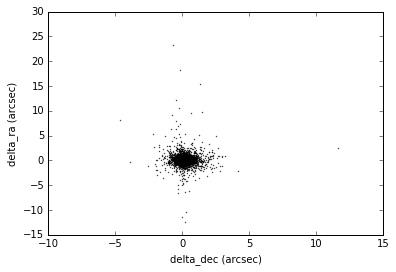
\includegraphics[width=0.4\textwidth]{astropy_match_ddec_vs_dra.png}}
		\subfigure[$J$  vs $\Delta \theta$]{
			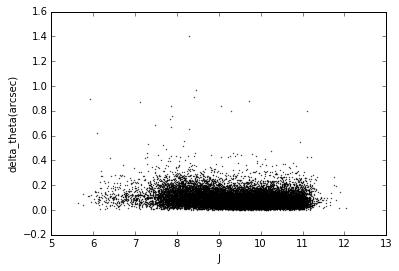
\includegraphics[width=0.4\textwidth]{astropy_match_J_vs_dtheta.png}}
		\caption{Cross-match result given by Scipy KDTree}
	\end{figure}
	
		\begin{figure}[H]
		\centering
		\subfigure[$\Delta ra$ vs $\Delta dec$]{
			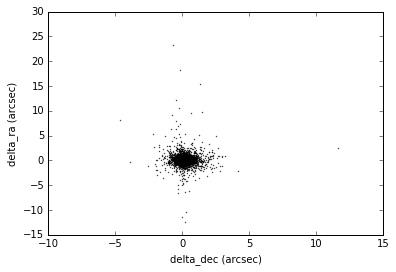
\includegraphics[width=0.4\textwidth]{self_match_ddec_vs_dra.png}}
		\subfigure[$J$  vs $\Delta \theta$]{
			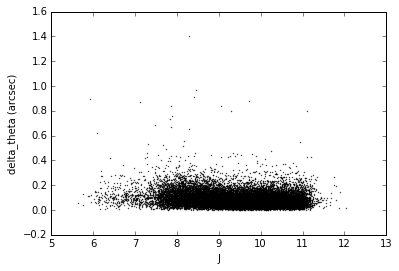
\includegraphics[width=0.4\textwidth]{self_match_J_vs_dtheta.png}}
		\caption{Cross-match result given by my KDTree}
	\end{figure}


\end{document}
